\chapter{Comparing $\delta$-electrons flagging algorithms}
\textit{This Chapter}
\section{Delta electrons}
One of the central challenges of Mu2e is the reconstruction of conversion electrons in the face of
large amounts of backgrounds from other known processes that follow muon capture by the
aluminum atoms. The detailed background rates for these processes at this energy scale are not very
well studied. In Mu2e, background rates calculated according to figures given in Nuclear Physics of
Muon Capture (D. F. Measday) are used to create simulations. However, due to the lack of
documentation at the energy scales involved in this experiment, there is a large uncertainty in
background rates which requires background removal to be insensitive to the level of backgrounds
This primary purpose of study is to address one prevalent source of background hits: the
secondary ionized electrons, which are referred to as "deltas." Deltas consist primarily of Compton
scattered electrons, pair production electrons, and delta rays, in order of decreasing prevalence.
Compton scattered electrons are produced when photons from various processes strike material
inside the detector. This causes the ejection of electrons that create the background events. The
photons primarily originate from neutron capture by atoms, which leads to an excited nuclear state
that decays via photon emission. These photons generally have energies on the order of a few MeV.
The neutrons, in turn, are created when muons are captured by atoms, creating unstable isotopes that
decay by ejecting neutrons. Pair production electrons, on the other hand, are produced when
processes involving nuclear recoil also produce pairs of electrons and positrons in order to conserve
energy and momentum. Delta rays, or secondary ionized electrons, are produced when charged
energetic particles collide with detector material.

\subsection{The Compton effect}
The Compton effect is the scattering of photons off quasi-free atomic electrons. 
In the treatment of this interaction process, the binding energy of
the atomic electrons is neglected. The differential probability of 
Compton scattering $\phi_c(E_\gamma, E^'_\gamma) dE^'_\gamma$ for $m_e c^2/2 < E^'_\gamma < E_\gamma$ 
is given by the Klein-Nishina formula:
\begin{equation}
    \phi_{\mathrm{c}}\left(E_\gamma, E_\gamma^{\prime}\right) \mathrm{d} E_\gamma^{\prime}=\pi r_e^2 \frac{N_{\mathrm{A}} Z}{A} \frac{m_e c^2}{E_\gamma} \frac{\mathrm{d} E_\gamma^{\prime}}{E_\gamma^{\prime}}\left[1+\left(\frac{E_\gamma^{\prime}}{E_\gamma}\right)^2-\frac{E_\gamma^{\prime}}{E_\gamma} \sin ^2 \theta_\gamma\right]
\end{equation}

where $\theta_\gamma$ is the scattering angle of 
the photon in the laboratory system (Figure \ref{fig:Compton}) and $E_\gamma$, $E^'_\gamma$
are the energies of the incident and scattered photon. 
\begin{figure}[!h]
    \centering
    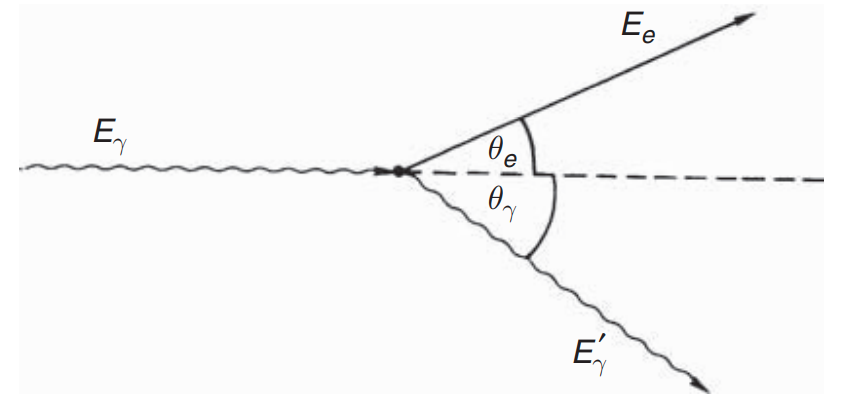
\includegraphics[width =0.6\textwidth]{figures/png/Screenshot_20240731_144138.png}
    \caption{}
    \label{fig:anglesinmuon}
\end{figure}


The total cross section for Compton scattering per electron is
given by [55]


The angular and energy distributions of Compton electrons are discussed
in great detail in R.D. Evans [56] and G. Hertz [48]. For the energy
spectrum of Compton electrons one gets

For Compton scattering off atoms the cross section is increased by the factor Z, because there are exactly Z electrons as possible scattering partners
in an atom; consequently σatomic
c = Z · σe
c .
At high energies the energy dependence of the Compton-scattering cross
section can be approximated by [57]

The ratio of scattered to incident photon energy is given by

Naturally, Compton scattering does not only occur with electrons, but
also for other charged particles. For the measurement of photons in particle detectors, however, Compton scattering off atomic electrons is of
special importance
\subsection{Pair production}
The production of electron-positron pairs in the Coulomb field of a
nucleus is only possible if the photon energy exceeds a certain threshold.
This threshold energy is given by the rest masses of two electrons plus
the recoil energy which is transferred to the nucleus. From energy and
momentum conservation, this threshold energy can be calculated to be

Since mnucleus  me , the effective threshold can be approximated by

If, however, the electron-positron pair production proceeds in the
Coulomb field of an electron, the threshold energy is

Electron-positron pair production in the Coulomb field of an electron is,
however, strongly suppressed compared to pair production in the Coulomb
field of the nucleus.
In the case that the nuclear charge is not screened by atomic electrons,
(for low energies the photon must come relatively close to the nucleus to
make pair production probable, which means that the photon sees only
the ‘naked’ nucleus),

\subsection{Energetic knock-on electrons ($\delta$ rays)}
The energy transfers to ionisation electrons can be so large that these
electrons can cause further ionisation. These electrons are called δ rays or
knock-on electrons. The energy spectrum of knock-on electrons is given
by [1, 10-12, 25]
dN
dEkin
= ξ · F
E2
kin
(1.25)
for I  Ekin ≤ Emax
kin .
F is a spin-dependent factor of order unity, if Ekin  Emax
kin [12]. Of
course, the energy spectrum of knock-on electrons falls to zero if the
maximum transferable energy is reached. This kinematic limit also constrains the factor F [1, 25]. The spin dependence of the spectrum of the
knock-on electrons only manifests itself close to the maximum transferable
energy [1, 25].
The strong fluctuations of the energy loss in thin absorber layers are
quite frequently not observed by a detector. Detectors only measure the
energy which is actually deposited in their sensitive volume, and this
energy may not be the same as the energy lost by the particle. For example, the energy which is transferred to knock-on electrons may only be
partially deposited in the detector because the knock-on electrons can
leave the sensitive volume of the detector.
Therefore, quite frequently it is of practical interest to consider only
that part of the energy loss with energy transfers E smaller than a given
cut value Ecut. This truncated energy loss is given by [10-12, 26]










The delta removal is a part of a series of selections on the hit properties to reduce background
hits.
The first selection concerns the energy deposited by the hit and excludes strongly ionizing
particles such as protons*. Since deltas aren't generally strongly ionizing, we require another selection
- hence this study. The last selection is made with respect to time. Namely, the time when the
conversion electron goes through the midpoint of the detector along the symmetry axis can be found
using an algorithm which takes the hits that pass the delta selection as input. By looking only at hits
within a short interval centered at this time, many background hits can be excluded.
In mu2e there are 2 types of rejections:
\begin{itemize}
    \item DeltaFinder
    \item FlgBkgHits
\end{itemize}


\subsection{Delta electron features}
Figure 2.1 shows the momentum distribution of deltas for 10,000 events.
Most deltas have much lower momenta than conversion electrons. This produces a significant
difference in their trajectories through the tracker, as shown in Figures 2.2 to 2.4. With the naked eye
one can already see dramatic differences.
The most striking quality of deltas is that they tend to create small, dense clusters of hits, as
shown in Figures 2.3 and 2.4. This motivates a "clustering approach"*: we search for such
concentrated clusters in the x-y plane using a clustering algorithm since deltas are very likely to reside
in such a cluster. However, the reverse containment does not hold - clusters can also contain many
conversion electron hits. Removing conversion electron hits can severely harm subsequent
reconstruction, so a filter is necessary. 
low energy (delta, compton, photon conversion) electrons are the largest source of the hits
in the tracker - about 2/3 of the total
language: $\delta$-electron - an electron with P<20 MeV/c
radius of a 10 MeV/c electron in the nominal Mu2e field < 3 cm, close to the resolution
along the wire
very specific topology - multiple hits with the same (X,Y) , within the resolution
\subsection{Hit Position Information and Clustering}
As mentioned above, the current straw drift tube position measurement limits the resolution to a
few cm. An improved position measurement can be made by taking advantage of the various layers of
straws that have large overlaps in the transverse plane. By taking two hit measurements from a pair of
intersecting straws and requiring them to be within a time window of on the order of the maximum
drift time*, one can reliably infer that such a pair of hits have been produced by the same particle and
occurred at the intersection of the two straws in the projected plane. Since the method involves two
dimensional information (from two straws), it is referred to as the stereo information method. Such a
measurement is much more precise, as shown in Figure 3.1.

\subsection{DeltaFinder}
step 1: Find $\delta$-electron track segments separately within each station
connect segments, allow 1 station wide "gaps"
dominant sources of failures:
I stations with MC particle producing hits in only one face;
I hits with wrong coordinates along the wire - long tails of the $\Delta$T distribution;
I recover hits in "empty" stations to improve efficiency;
I optimization of the algorithm timing performance;
electron hit energy dependence on momentum: path length within the straw depends on momentum
only about 4\% of CE hits have energies above 3.5keV (1\% above 5 keV)
consider several hit energy cutoffs: 3.5 keV, 5keV, 7keV, use all hits
\subsection{FlgBkgHits}
flgbkg flags hits with high charge

\section{Analysis}
The Mu2e Simulation framework is described in Appendix \ref{mu2eana}
